\documentclass[runningheads]{llncs}

%PACKAGES
\usepackage[utf8]{inputenc}
\usepackage{listings, xcolor}
\usepackage{graphicx} 
\usepackage{lipsum}
\usepackage{float}
\setcounter{secnumdepth}{5}
\begin{document}
\title{Comparing FreeST, Go and Rust}
\author{Jorge Martins\inst{1} \and
Diogo Lopes\inst{1}
}
\definecolor{darkblue}{rgb}{0.0, 0.0, 0.55}
\lstset{language=Java,
numbers=none,
keywordstyle = \color{blue},
commentstyle = \color{darkblue},
breaklines = true,
showstringspaces = false,
tabsize = 4,
basicstyle=\small,
} 
\institute{Departamento de Informática da Faculdade de Ciências da Universidade de Lisboa
\email{\{fc51033,fc51058\}@alunos.fc.ul.pt}}
\nocite{*}
\maketitle
\thispagestyle{empty}
\begin{abstract}
FreeST is an experimental functional programming language being developed at LASIGE that offers primitives to thread creation and channel communication, different to those in programming languages such as Go and Rust, that are currently being appraised by their performance and reliability. Despite being different, these languages are comparable by the characteristics of their common primitives and by their learning curve. Although there a several articles comparing Rust and Go, they mainly focus in performance and reliability instead of the learning curve of each language and their channels and thread creation primitives. FreeST on the other hand, due to the small community working on it, is yet to be compared to the others.
In order to compare the three languages we used a algorithm that focus on thread creation, communication using channels and thread synchronization using those same channels and learned the three languages in order to comment on the difficulties and different aspects of each.
This comparison is useful to understand what aspects of some languages could benefit the others and also to inform about what difficulties one may find when writing code in each of them.
\end{abstract}
\section{Introduction}
Rust and Go are languages that are growing in popularity due to their performance and reliability, according to the TIOBE index. FreeST\cite{freest} on the other hand is very recent programming language being developed at LASIGE, a research center in the Faculty of Sciences of the University of Lisbon.
In order to compare the three languages, that were completely new to each of us until the start of this project, we aimed to understand the basic concepts of each language, such as the ownership and lifetimes in Rust or the session types \cite{session} in FreeST.
%TODO something here
Our goal was to implement a simple communication algorithm that simulates a conversation between a customer and an agency selling plane tickets in Rust, Go and FreeST, understanding the main differences and characteristics of each language and identifying the main complications we felt when learning them.
\newpage
\section{Background}
\subsection{The Plane Ticket Algorithm}
In order to explore the interprocess communication through channels and thread creation, we used a simple algorithm that simulates a customer trying to buy a plane ticket from a agency.
\begin{figure}[H]
\centering
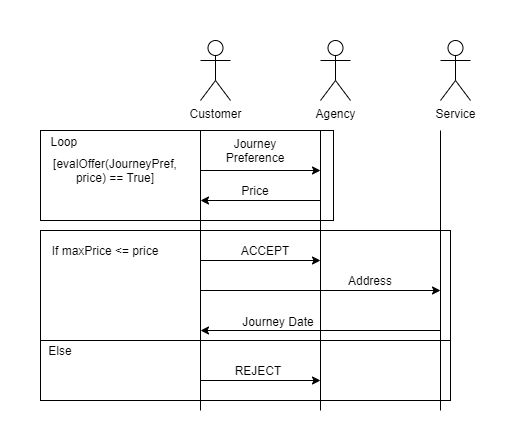
\includegraphics[scale=0.4]{Algorithm.png}
\caption{Plane Ticket Algorithm System Sequence Diagram}
\label{ssd}
\end{figure}
As we can see in figure \ref{ssd} the algorithm consists in an early stage of negotiation where a customer will send a journey preference(e.g. "Rome") to the agency and receive the price for a ticket to the given preference repeatedly until evalOffer evaluates to true.
At this point the customer will make a choice:
\begin{itemize}
\item If the received price is lower or equal to the max accepted price of the customer, he will accept the offer.
The agency will spawn a service which will receive the customer address and send the journey date.
\item If the received price is greater than the max accepted price of the customer, he will reject the offer and end the communication.
\end{itemize}
The pseudo code for this algorithm is as follow:
\begin{lstlisting}[caption={Customer Algorithm},captionpos=b]
class Customer {
	Address addr;
	double price, maxPrice;
	bool loop := true;
	String journeyPref;
	new Agency.sell {
		sendWhile (loop) {
			send( journeyPref );
			price := receive;
			loop := evalOffer(journeyPref,price);
			// implementation of evalOffer omitted
		};
		sendCase( evalPrice(price,maxPrice) ) {
			ACCEPT > send( addr ); Date date := receive;
			REJECT > null; /* customer rejects price
					,end of protocol */ 
		}
	} /* End method invocation */
}
\end{lstlisting}
\begin{lstlisting}[caption={Agency Algorithm},captionpos=b]
class Agency {
	String journeyPref;
	void acceptOrder sell {
		receiveWhile {
			journeyPref := receive;
			double price := getPrice( journeyPref );
			// implementation of getPrice omitted
			send( price );
		}
		receiveCase (x) { // buyer accepts price
			ACCEPT < new Service . orderDelivery { } ,
			REJECT < null;// receiveCase : buyer rejects 
        }
	} /* End method sell */
}
\end{lstlisting}
\begin{lstlisting}[caption={Service Algorithm},captionpos=b]
class Service {
	void receiveOrderSession orderDelivery() {
		Address custAddress := receive;
		Date date := new Date();
		send( date );
	}
}
\end{lstlisting}
\subsection{Programming Languages}
\subsubsection{Rust}\hfill\\\\
\subsubsection{Go}\hfill\\\\
\subsubsection{FreeST}\hfill\\\\
\lipsum[1]
\section{Implementation Details}
\lipsum[1]
\subsection{Go}
\lipsum[1]
\subsection{Rust}
\lipsum[1]
\subsection{FreeST}
\lipsum[1]
\subsection{Discussion}
Here you should discuss the results on a high level. For instance, based on our results, the parallelization of the merge-sort is relevant as no other parallel work occurs at the same time, and the complexity $O(N log(N))$ can have a large impact when the number of individuals is high.
\section{Conclusions}
Here you should resume the major conclusions taken from discussion. Ideally, these should align with the objectives introduced in the introduction.


You should also list the future work, i. e., tasks and challenges that were outside your scope, but are relevant.
\section*{Acknowledgements}
First Author wrote the part of the program implemented the phasers. Second Author implemented the MergeSort in parallel. 

Both authors wrote this paper, with First Author focusing on the introduction, related work and conclusions while the Second Author focused on approach and evaluation.

Each author spent around 30 hours on this project.
\bibliographystyle{unsrt}
\bibliography{bibliography}
\end{document}